% v2-acmsmall-sample.tex, dated March 6 2012
% This is a sample file for ACM small trim journals
%
% Compilation using 'acmsmall.cls' - version 1.3 (March 2012), Aptara Inc.
% (c) 2010 Association for Computing Machinery (ACM)
%
% Questions/Suggestions/Feedback should be addressed to => "acmtexsupport@aptaracorp.com".
% Users can also go through the FAQs available on the journal's submission webpage.
%
% Steps to compile: latex, bibtex, latex latex
%
% For tracking purposes => this is v1.3 - March 2012

\documentclass[prodmode,acmtosem]{acmsmall} % Aptara syntax

% Package to generate and customize Algorithm as per ACM style
\usepackage[ruled]{algorithm2e}
\usepackage{textcomp}
\usepackage{gensymb}
\usepackage[utf8]{inputenc}
\usepackage[table]{xcolor}
\usepackage{natbib}
\usepackage{subfigure}
\renewcommand{\algorithmcfname}{ALGORITHM}
\SetAlFnt{\small}
\SetAlCapFnt{\small}
\SetAlCapNameFnt{\small}
\SetAlCapHSkip{0pt}
\IncMargin{-\parindent}

% Metadata Information
% \acmVolume{9}
% \acmNumber{4}
% \acmArticle{39}
% \acmYear{2010}
% \acmMonth{3}

% Copyright
%\setcopyright{acmcopyright}
%\setcopyright{acmlicensed}
%\setcopyright{rightsretained}
%\setcopyright{usgov}
%\setcopyright{usgovmixed}
%\setcopyright{cagov}
%\setcopyright{cagovmixed}

% DOI
%\doi{0000001.0000001}

%ISSN
%\issn{1234-56789}

% Document starts
\begin{document}

% Page heads
\markboth{}{Dynamic obstacle mapping for the visually impaired using sensor fusion.}

% Title portion
\title{Dynamic obstacle mapping for the visually impaired using sensor fusion.}
\author{Johann Thor Kristthorsson
\affil{University College London}
Ifeanyi Ndu
\affil{University College London}
Veselin Pavlov
\affil{University College London}
Shuang Zhang
\affil{University College London}
}
% NOTE! Affiliations placed here should be for the institution where the
%       BULK of the research was done. If the author has gone to a new
%       institution, before publication, the (above) affiliation should NOT be changed.
%       The authors 'current' address may be given in the "Author's addresses:" block (below).
%       So for example, Mr. Abdelzaher, the bulk of the research was done at UIUC, and he is
%       currently affiliated with NASA.

\begin{abstract}
Abstract goes here
\end{abstract}


%
% The code below should be generated by the tool at
% http://dl.acm.org/ccs.cfm
% Please copy and paste the code instead of the example below. 
%
% \begin{CCSXML}
% <ccs2012>
%  <concept>
%   <concept_id>10010520.10010553.10010562</concept_id>
%   <concept_desc>Computer systems organization~Embedded systems</concept_desc>
%   <concept_significance>500</concept_significance>
%  </concept>
%  <concept>
%   <concept_id>10010520.10010575.10010755</concept_id>
%   <concept_desc>Computer systems organization~Redundancy</concept_desc>
%   <concept_significance>300</concept_significance>
%  </concept>
%  <concept>
%   <concept_id>10010520.10010553.10010554</concept_id>
%   <concept_desc>Computer systems organization~Robotics</concept_desc>
%   <concept_significance>100</concept_significance>
%  </concept>
%  <concept>
%   <concept_id>10003033.10003083.10003095</concept_id>
%   <concept_desc>Networks~Network reliability</concept_desc>
%   <concept_significance>100</concept_significance>
%  </concept>
% </ccs2012>  
% \end{CCSXML}

% \ccsdesc[500]{Computer systems organization~Embedded systems}
% \ccsdesc[300]{Computer systems organization~Redundancy}
% \ccsdesc{Computer systems organization~Robotics}
% \ccsdesc[100]{Networks~Network reliability}


\keywords{Sensor Fusion, Software Engineering,
Visually Impaired, Blind, Microsoft}

\acmformat{Johann Thor Kristthorsson, Ifeanyi Ndu, Veselin Pavlov and Shuang Zhang, 2016.}


\begin{bottomstuff}
This work was made in collaboration with Microsoft and the Guide Dogs association.
\end{bottomstuff}

\maketitle

\section{Introduction}
There are two million people living with visual impairment in the UK and despite that fact indoor environments are often not designed with this large group of people in mind. ~\cite{NHSBlindStatistics} This means that the visually impaired have to depend on mobility tools to make their way around their environment. Mobility canes and guide dogs are the most important ones but are limited in their use. The canes have limited use to a person needing to navigate from place to place and the guide dogs are not currently available to assist all visually impaired persons in the UK. The Guide Dogs Association is working towards the goal of providing as many people with guide dogs as possible but are not able to meet demand. The project falls under the Cities Unlocked umbrella, an initiative that was started to respond to the lack of available guide dogs in the UK ~\cite{CitiesUnlockedGeneral}. Cities Unlocked has recently been moving more towards improving and enriching the experiences of the visually impaired, rather than focusing solely on their mobility.

Microsoft has been exploring different technologies that could help the visually impaired in their day to day lives and wanted to elicit the help of UCL in this exploration. A team of 8 MSc students, 4 from software systems engineering and 4 from computer science, was put together and that team took Microsoft and the Guide Dogs Association on as clients for this project. To clarify the specific topic of the project several brainstorming sessions were held to explore the aims and goals. The specific field of study that the clients wanted the team to explore was the use of wearable sensors that could be used by the visually impaired. Additionally the clients wanted to use cheap, off the shelf, hardware and use a technique called Sensor Fusion to maintain accuracy.
After exploring several possible use cases for these technologies the client and the UCL team decided to find a way to improve the experience of the members of the visually impaired population when entering specific indoor environments.
Specifically in environments that are unfamiliar to the user and that are not equipped with any specific navigation infrastructure. There has already been thorough research done on indoor navigation but the identification of obstacles seemed to be a good fit for the hardware and technology requirements of the client.

\section{Literature review} % TODO: Change to background
% TODO: Check if there is a difference in font size.
% TODO: use the 
% TODO: citet and citep
Obstacle detection is a large topic and has been popular in the last few years with the advent of autonomous vehicles and unmanned aerial vehicles.
The Defence Advanced Research Project Agency (DARPA) in the United States has held several competitions to push the research community towards this specific topic. The DARPA Grand Challenge in 2005 and the Urban Challenge in 2007 offered millions of dollars in prizes and sparked great interest within the research community~\cite{DARPAGrandChallenge2005,DARPAUrbanChallenge2007}.
\subsection{Obstacle detection}
In the specific case of obstacle detection as an assistive technology there have been several papers exploring the topic. \citet{Cardin2007} developed a wearable system that uses an array of ultrasonic transducers to do sonar sensing of obstacles around a subject. The subject is notified of the obstacles through vibrotactile instruments sewn into clothing around the subjects torso. Experiments were conducted by blindfolding test subjects and having them navigate an environment filled with obstacles. The time it took the subjects to navigate was recorded and the use of the system resulted in a 50\% reduction in navigation time after a short training time~\cite{Cardin2007}. The system developed by \citet{Shin2007} is similar to \citet{Cardin2007} but adds audible feedback through a headset~\cite{Shin2007}. These methods are entirely reactive, in that they sense and identify obstacles in a space but do not record its position for possible future use. In addition to this the evaluation of the detection accuracy is lacking. The studies do not describe their experimental setups accurately and the data collection methods are never mentioned. 
%These types of methods are common and widely explored both for the purposes of small robots and autonomous vehicles ~\cite{Kato2002}. 
%Shoval et al. have made attempts to fuse the work done in autonomous driving and robotics with the work in assistive technologies. They did this by mounting sonar sensing hardware on a robot that serves the same purpose as a guide dog. It has one axle and wheels that are powered. The robot is pushed by the subject via a handle, the robot can then detect and avoid obstacles and the subject notices the change in the robots movements through the handle ~\cite{Shoval2003}.
\subsection{Sensor Fusion}
Sensor fusion, or cooperative fusion, is a well known term in the context of obstacle detection and navigation. \citet{Labayrade2005} describe algorithms and architectures that facilitate cooperative fusion of two different kinds of sensors, stereovision and LIDAR to detect obstacles in an autonomous driving scenario~\cite{Labayrade2005}. Cooperative fusion is used to detect obstacles in the road in front of a vehicle and determine its distance with good accuracy. The use of sensor fusion decreased the rate of false negatives in the detection from 14.7\% and 5.2\% for LIDAR and stereovision respectively, down to 5.2\%. In addition the rate of false negatives went down from 4.5\% and 3.2\% respectively to 1.2\%. \citet{Cho2014} reached similar results showing an increase in the rate of true positives in obstacle detection from 83.2\% to 89.9\% by using fusion instead of using actual sensor values~\cite{Cho2014}. Contrary to the research found for the use cases for the visually impaired these papers provide a thorough explanation of the evaluation and data gathering performed and will proved useful in designing the evaluation strategy for this project. These methods have been developed specifically for use in the scenario of autonomous driving but are directly applicable to the scenario of detecting obstacles around a visually impaired pedestrian. Sensor Fusion was introduced into window 8 Operating system to provide stability to applications relying on clean and stabilised data. \citet{Gear2012} described a situation where Engineers at Microsoft attempted to map a 3D virtual environment to a real Environment in an app through a tablet. First of all they tried emulate up and down movements in the virtual environment using an accelerometer. Almost immediately they encountered an issue when tilting the tablet and holding the tablet in a stationary position. Noise coming from the accelerometer alone caused jittery movements in the applications. To achieve a much more stable movement, the accelerometer readings was passed through a low-pass filter. The low-pass filter fulfilled its duty but simultaneously introduced a bottleneck into the app. Movement was significantly smoother but the motion in the app felt unresponsive and sluggish. The engineers also used a 6-axis compass which is a 3D accelerometer and 3D magnetometer to emulate left and right movements however it did not yield practicable result due to the instability of the 6-axis sensor. Finally the engineers hit a breakthrough with sensor fusion using the 3D accelerometer, 3D magnetometer and 3D gyroscope. Data collected from all 9-axis resulted in a smooth and fluid experience in the virtual app. Additionally the sensors complemented each other in terms of areas where they fell short~\cite{Gear2012}.
In light of research described in the literature reviewed the team will be able to reach the aforementioned aims of this project by developing a data collection platform that gathers data from many different cheap sensors. The sensor data will be used to identify obstacles and the accuracy of the results will be increased by using sensor fusion.



% Add aims and goals
% What are we building now and what are it's aims
\section{Proposed System}
% TODO: make a good argument for how we managed RISK
\subsection{Preliminary work}
% How did we end up with our current aim
% US sensors and why we discarded those.

% Subsection this into VI obstacle detection and Sensor fusion, then bring back together.

%TODO: citation 

The initial plan for this project was to make use of hardware developed by students in the Electrical Engineering department. The hardware consists of an armband that can detect ultrasonic frequencies. Those frequencies are emitted by at least 3 beacons in strategically predefined locations in the room. The armband, in conjunction with a computer and an Android device, then triangulates the position of the armband in space.\\\\
The use cases that were to be explored were centred around detecting gestures and possible indoor location possibilities. However, soon after the project was presented to the team the hardware was found to have several limitations. The team found that the location accuracy was considerably less than what was initially described. The initial description of the hardware stated that the location accuracy was sub-centimetre, which is the theoretical minimum, but the functional accuracy was between 10 and 50 centimetres. This eliminates the gesture use case since more accuracy is needed to get accurate gesture recognition.
%TODO: citation
Furthermore the hardware can only functions if 3 beacons are within a 130\degree cone in front of the receiver. This severely limits the practicality of the device for indoor location since a wearable piece of hardware is usually blocked by the wearers body in addition to any obstacle in the environment such as static or movable objects.\\\\
%TODO: citation
Our initial contact with the client was a brainstorming session where he expressed his vision for the project. He expressed his desire to have an end product which would feel natural to the user with very little work on the user's part in terms of learning getting themselves familiar with the product. Then he raised the idea of using a sensor or combination of wearable sensors to achieve the ultimate goal. Ideas were then bounced around and a subject area was found that was open for research and of value to our client.\\\\
Microsoft Research have done some investigation into using Sensor Fusion
%TODO: citation
and wanted to see what applications for that technology in aiding the visually impaired. 

After the meeting the team met several times to brainstorm and research possible applications around the sensor fusion concept and decided on a few possible project proposals.
These were presented to the client and he expressed interest in continuing with one of them.\\\
For the final project proposal our client agreed on a research area that will help the visually impaired navigate an indoor environment.
Using sensor fusion the team was to build a system that can collect data from various disparate sensors and identify the location of the user and obstacles in its environment.
The goal is to use cheap, of-the-shelf sensors and mitigate any error in the sensor readings by correlating different readings. This will help us reduce error and increase accuracy by using various sensor fusion methods.
\subsection{High level goals}


\subsection{Requirements}

Table \ref{table:1} shows a list of requirements our system will fulfil (please see section \ref{Appendix} for a full description of our requirement patterns).\\

\renewcommand{\arraystretch}{1.5}

\begin{center}
\begin{tabular}{| l ||} 
 \hline
 \rowcolor{lightgray}\multicolumn{1}{c}{List of Requirements} \\ [0.5ex] 
 \hline\hline
 Identifying points of interest in the environment. \\ 
 \hline
 Detecting obstacles \\
 \hline
 Feeding back mapping information \\
 \hline
 Manually identifying obstacles in a space \\
 \hline
 Manually removing an obstacle from the map \\ 
 \hline
 Providing navigation for a user to a point of interest \\ 
 \hline
 Voice interactions - listing \\ 
 \hline
 Voice interactions - acceptance \\ 
 \hline
 Screen interactions - listing \\ 
 \hline
 Screen interactions - acceptance \\ 
 \hline
 Classification of obstacles/Points Of Interest \\ 
 \hline
 3D Directional Sound \\ 
 \hline
 Head Gestures \\ 
 \hline
 IR and Ultrasound \\ 
 \hline
 Machine Vision \\ 
 \hline
\end{tabular}
\label{table:1}
\end{center}

\section{System Architecture}
\label{architecture}
Given the goals the team and the client set for this project there were several considerations to be made to make the architecture flexible and performant enough to satisfy the requirements. Having the requirement of being able to accept data from many kinds of sensors made it clear that the architecture had to be made up of a variety of strategies to homogenise the data so that it could be processed in a more abstract way. Subsequent processing could then be performed based on a fixed data model that would make it easier to rapidly develop and evaluate different processing strategies.

\subsection{Data collection}
Since data reaching our platform will be produced from various sources, it was of paramount importance that we build a system whereby huge amount of data can be collected and aggregated for further processing as at when needed. After much consideration, we decided to include Apache Kafka and Apache Zookeeper into our overall System Architecture. Apache Kafka is a distributed publish/subscriber message queuing system that provides fault tolerance, high throughput for both publishing and subscribing tasks, supports multiple consumer, holds messages on disk for latter consumption in bulk and could also be used as a commit log service. Apache Zookeeper is a service that provides synchronization across a cluster in a distributed network. Zookeeper assists kafka in maintaining order across a Kafka cluster, it maintains properties such its configuration and leader election should a leader in the cluster fails to exist. Both Apache Kafka and Apache Zookeeper have the capability of scaling out. Additional kafka brokers can be added to the cluster depending on the requirements of the architecture, as well as additional zookeeper servers can be included but will have a master zookeeper server to oversee events in the distributed zookeeper network.

\subsection{Aggregation} 
Apache Kafka and Apache Spark

\subsection{Processing}
Apache Spark

\subsection{Feedback}
I think Android App?

% TODO: make a good argument for how we managed RISK

\section{Implementation}
As described in section~\ref{architecture} the chosen architecture uses a variety of different technologies to achieve its goal. Each component therefore had a predefined best practice in implementation. The team aimed to follow best practices when working with each technology and align their work so that each member would be able to work on each component interchangeably.

Before diving into suitability arguments for chosen architecture, it would be of immense importance to discuss how components in our architecture will interact with each other. A socket on our VPS will be listening indefinitely on a particular port for incoming data from our various sensing hardware. Each sensor or combination of sensors will measure data, do some preprocessing before sending data across to our VPS over a UDP connection. For instance one of the CS students would send three distance estimates based on the measurements collected from 2 ultrasound and 1 infrared sensor. At the listening end we would essentially do a partial deserialisation to obtain the topics from each packet. Afterwards the packet 

% Why Java for 

\subsection{Technology}

% Architecture here
% TODO: Reevaluate the structure here
\section{Project Management}
% Discuss 
The team consists of 8 Masters students, 4 are doing a conversion course in Computer Science and 4 are doing Software Systems Engineering. As discussed earlier the 4 CS students are each responsible for a data collection or feedback application that would be the topic of their dissertation project.
The role of the SSE team with regards to the CS students was to coordinate their efforts towards creating value for the client and to provide them with guidance with the implementation and architecture of their projects.

\subsubsection{Processes}
Describe tools and processes, Scrum, Kanban etc.

\subsection{Tools}
Jira, Slack Maybe not needed.

\subsubsection{Communication}
Talk about our communication and meeting schedule.

\subsection{Testing strategy}
Show how our integration and load testing evaluates our architecture and a discussion of why it fits well

\section{Evaluation}
Metrics and graphs showing the performance of certain parts of the project.

\begin{figure}
\centering
\subfigure[Figure 1] {
  \label{fig:sub1}
  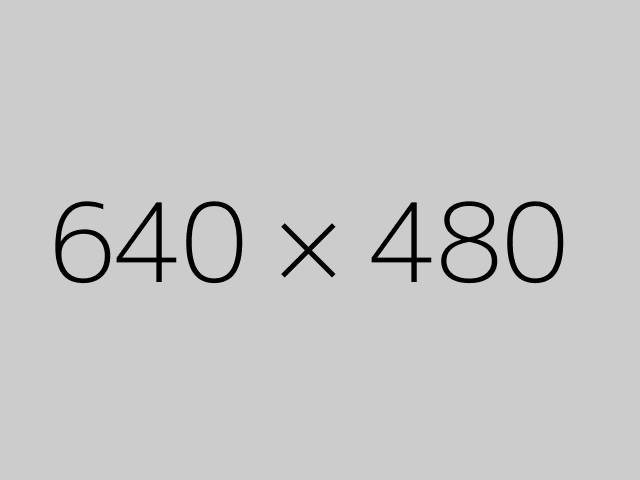
\includegraphics[width=.3\linewidth]{test640}
}
\subfigure[Figure 2] {
  \label{fig:sub1}
  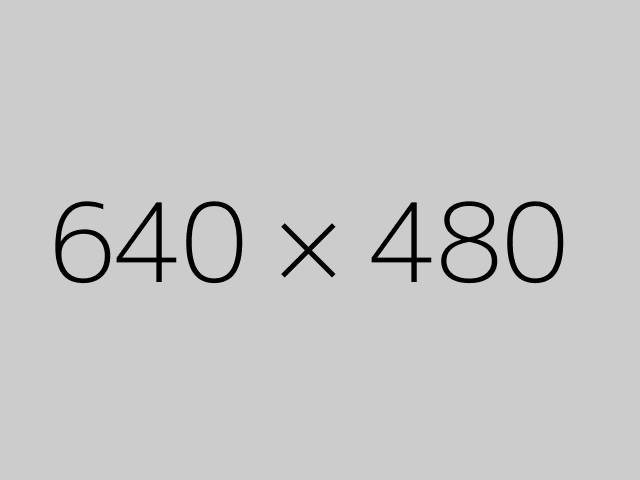
\includegraphics[width=.3\linewidth]{test640}
}
\subfigure[Figure 3] {
  \label{fig:sub1}
  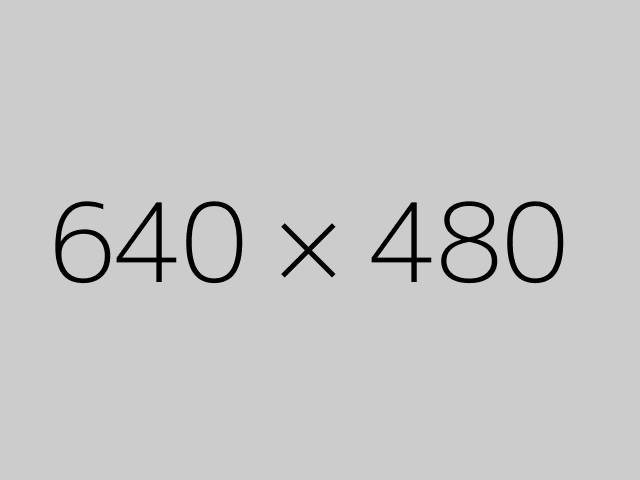
\includegraphics[width=.3\linewidth]{test640}
}
\caption{A figure with two subfigures}
\label{fig:test}

\subfigure[Figure 4] {
  \label{fig:sub1}
  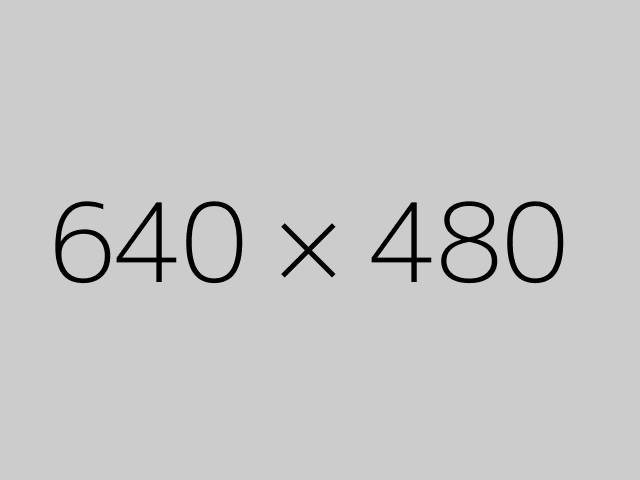
\includegraphics[width=.3\linewidth]{test640}
}
\subfigure[Figure 5] {
  \label{fig:sub1}
  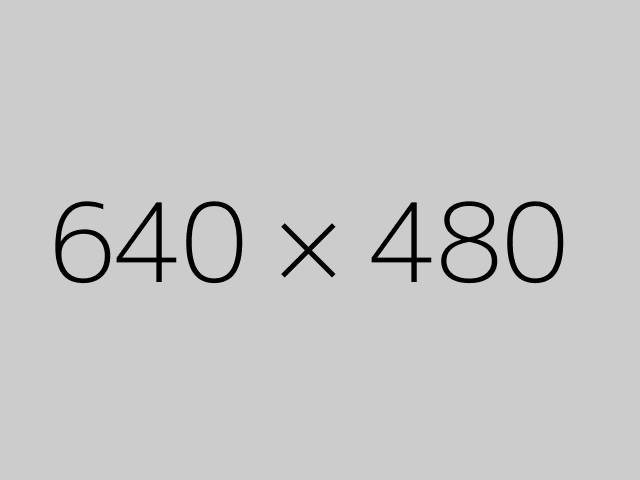
\includegraphics[width=.3\linewidth]{test640}
}
\subfigure[Figure 6] {
  \label{fig:sub1}
  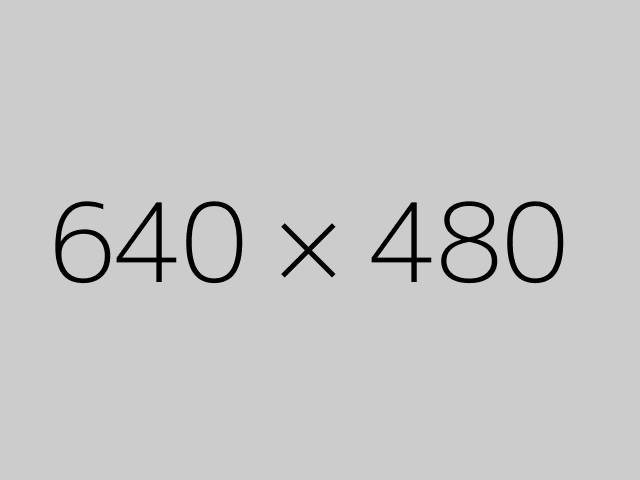
\includegraphics[width=.3\linewidth]{test640}
}
\caption{A figure with two subfigures}
\label{fig:test}
\end{figure}

\section{Life cycle and Future Work}
\subsection{Current state}
Describe the current state of the project\\
Capabilities, how many of the Goals and Requirements have been fulfilled.\\
Quality requirements and the tests we used to evaluate them\\

\subsection{Maintenance and Scaling}
% TODO: Enumerate limitation of the product
% TODO: Describe how we can go from prototype to a running system
% TODO: Add confidential appendix to report that does not go to the client.
Describe how the project can be maintained and scaled in the event of deployment.\\
Talk about the migration plan to Azure.\\


\section{Conclusions}

% TODO: identify the topic takeaway messages.
% takeaway messages describe how we one could do things differently.
% not in context of the project but rather in the context of the domain. 

% Appendix
\appendix
\section*{APPENDIX} \label{Appendix}
\setcounter{section}{1}

\appendixhead{ZHOU}

% Acknowledgments
\begin{acks}
\end{acks}  

% Bibliography
\bibliographystyle{ACM-Reference-Format-Journals}
\bibliography{GroupReport-bibfile}

% History dates
%\received{February 2007}{March 2009}{June 2009}

% Electronic Appendix
\elecappendix

\medskip

\section{This is an example of Appendix section head}


\section{Appendix section head}

\end{document}


